\documentclass[10pt,hyperref={CJKbookmarks=true},xcolor=dvipsnames,aspectratio=169]{beamer}
\usetheme[navigation]{UMONS}
\usepackage[utf8]{inputenc}
\usepackage{verbatim}
\usepackage{ctex}

\title[国际经济学]{国际经济学}
\subtitle{短期汇率决定理论:货币分析法}
\author{鲁晓东}
\institute[]{%
	岭南学院\hspace{2em}中山大学
	\\[4ex]
	
\includegraphics[height=8ex]{fig/lingnanlogo}\hspace{2em}%
	
\includegraphics[height=8.5ex]{fig/sysu}
}
%------------section前展示一页----------
\AtBeginSection[] {     
	\begin{frame}        
	\tableofcontents[currentsection,hideallsubsections]    
\end{frame} 
}

%-------------subsection也展示一下----------
\AtBeginSubsection[]{

\frame<beamer>{ 
	
	\frametitle{Outline}   
	
	\tableofcontents[currentsection,currentsubsection] 
	
}

}
%---------------------------

%-----------一段一闪现-------
%\beamerdefaultoverlayspecification{<+->}
%这个功能基本不用

\begin{document}
\maketitle


\begin{frame}
\frametitle{提纲}
\tableofcontents
\end{frame}				%生成提纲页

%-----------正文开始----------------------



\section{Motivation }
\begin{frame}{Motivation}
\begin{columns}
	\begin{column}{0.7\textwidth}
		
		\begin{itemize}[<+->]
			\small
			\item 基于fx是一种资产的思想,UIP和CIP分别提出一种即期汇率和远期汇率的决定机制。无论是UIP和CIP理论,利率都居于核心地位。
			\item 那么利率又是由什么来决定的呢?
			\item 如果利率是由货币的供求来决定的,那么一国的货币供求存量的相对变化可以解释汇率的变动
			\item 基于以上逻辑,货币主义学派提出一系列模型来解释汇率的变动(例如弹性价格模型、粘性价格模型、实际利差模型等)
			\item 以上模型的共同点是假定本国债券和外国债券能够完全替代,也就是说影响对它们相对供求的因素只有一个:利率差异。如果允许本国债券和外国债券存在风险差异,则会把我们引向——\structure{资产组合平衡模型}
			
		\end{itemize}
	\end{column}
\begin{column}{0.3\textwidth}
	\centering
	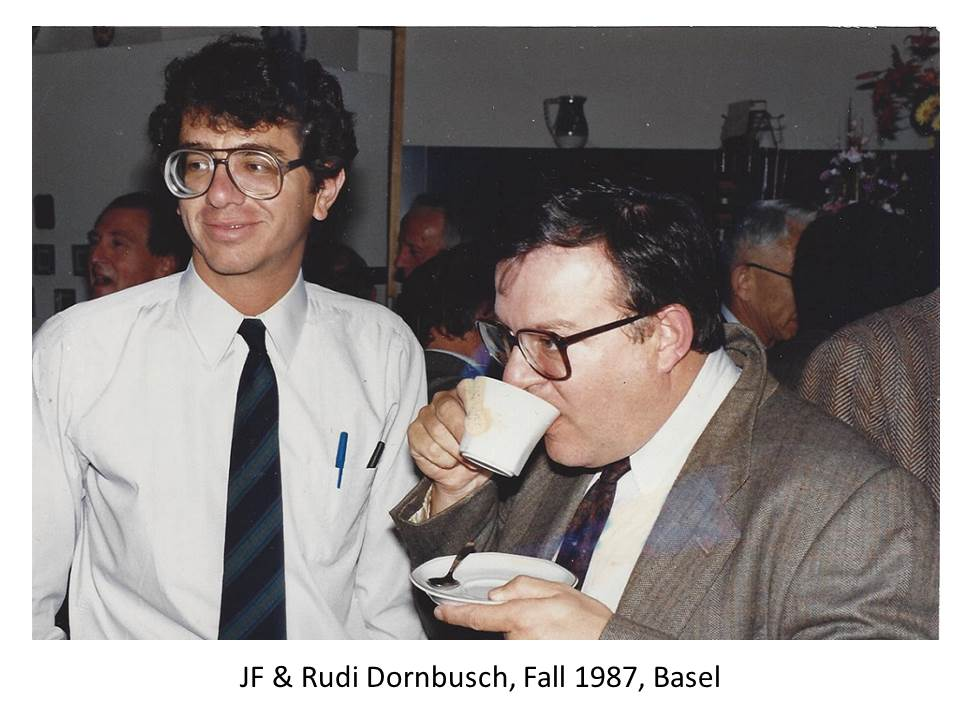
\includegraphics[scale=0.2]{fig/shortrunexchange/dornbusch}
\end{column}
\end{columns}


\begin{block}{Monetarism货币主义}

	\textcolor{red}{Monetarism} is a school of thought in monetary economics that emphasizes the role of governments in controlling the amount of money in circulation. Monetarist theory asserts that variations in the money supply have major influences on national output in the short run and on price levels over longer periods. 
\end{block}
\end{frame}

\frame{% how to print
	\frametitle{}
	\begin{center}
		\textcolor{blue}{Chapter 15: Money, Interest Rates, and Exchange Rates}
	\end{center}
}

\frame{
	\frametitle{Money}
	\begin{itemize}
		\item Why do we need it?
		\begin{enumerate}
			\item Medium of exchange
			\item Unit of account
			\item Store of value
		\end{enumerate}
	\end{itemize}
}

\section{复习:货币与利率的决定}
\frame{
	\frametitle{Money - Medium of exchange}
	\begin{itemize}
		\item Mutual cooincidence of wants
		\begin{itemize}
			\item I want a bottle of water right now
			\item 7-Eleven needs economic analysis right now
		\end{itemize}
		\item Unlikely\dots 
		\item Money helps us:
		\begin{itemize}
			\item Avoid complicated barter exchanges
			\item Automatically get the value of our own production
			\item When we buy something, it is as if we had bartered
		\end{itemize}
	\end{itemize}
}

\frame{
	\frametitle{Money - unit of account}
	\begin{itemize}
		\item Comparing values of different things
		\item Thought experiment
		\begin{itemize}
			\item Suppose that the prices at the canteen in 学一 were all in bananas 
			\item Suppose that the prices at the canteen in 学五 were all in toothbrushes 
			\item For ex: Coke costs 10 bananas at SP, and 2 toothbrushes at P
			\item Where is it more expensive?
		\end{itemize}
		\item Money helps us:
		\begin{itemize}
			\item Quickly compare prices across goods and locations
		\end{itemize}
	\end{itemize}
}

\frame{
	\frametitle{Money - Store of Value}
	\begin{itemize}
		\item Money is an asset
		\begin{itemize}
			\item If you want, keep in under your mattress!
		\end{itemize}
		\item It is the most liquid asset, a benchmark
	\end{itemize}
}

\frame{
	\frametitle{What is money?}
	\begin{itemize}
		\item More difficult question than it seems!
	\end{itemize}
\centering
	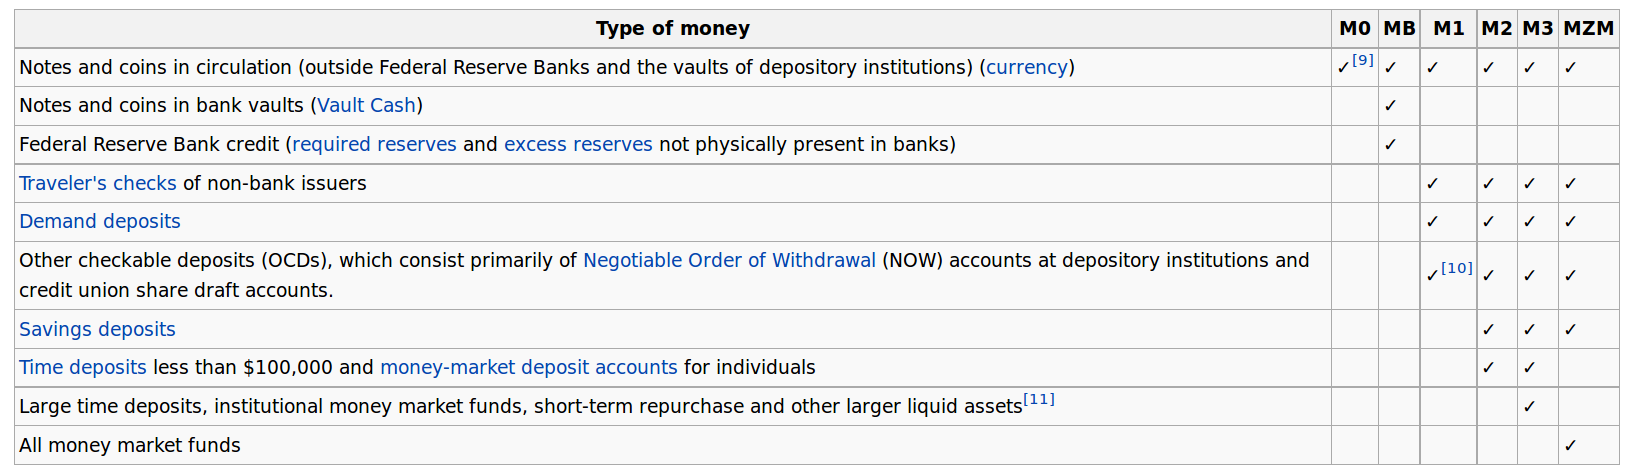
\includegraphics[scale=0.25]{fig/shortrunexchange/money_supply.png}
	\begin{itemize}
		\item M1 is the most liquid
		\item In this book, \emph{money supply} is M1
	\end{itemize}
}

\frame{
	\frametitle{A difficult quesiton}
	\begin{itemize}
		\item Money does three things
		\begin{enumerate}
			\item Medium of exchange
			\item Unit of account
			\item Store of value
		\end{enumerate}
		\item Why do we use pieces of paper and not gold coins?
		\item Or at least pieces of paper that could be redeemed for gold 
		\begin{itemize}
			\item What is the advantage we get from paper?
			\item Gold has an advantage: independent value\dots
		\end{itemize}
		\item Bitcoin\dots
	\end{itemize}
}

\frame{
	\frametitle{Money Supply \& Demand}
	\begin{itemize}[<+->]
		\item \textbf{money supply} controlled by Central Bank 
		\begin{itemize}
			\item Actually process a bit complicated, see Chpt. 18
			\item For now just assume M1 chosen by Central Bank
		\end{itemize}
		\item \textbf{money demand} represents the amount of monetary assets that people are willing to hold. This is based on:
		\begin{enumerate}[<+->]
			\item Interest rates/expected rates of return 
			\item Risk/inflation
			\item Liquidity
		\end{enumerate}
	\end{itemize}
}

\frame{
	\frametitle{Expected return and interest}
	\begin{itemize}
		\item M1 pays no interest (to a first approximation)
		\item If hold cash, lose interest gained by holding illiquid asset
		\item The higher the interest rate, the higher opportunity cost of holding cash
		\begin{itemize}
			\item One safe way of earning interest is a risk-free bond
			\item Classic example, American T-Bill
			\item The higher the return on T-Bill, the less demand for cash
		\end{itemize}
	\end{itemize}
}

\frame{
	\frametitle{Risk}
	\begin{itemize}
		\item Textbook claims risk is not important
		\item Argument, all financial assets are denoted in currency
		\item Can't insure against risk
		\item I'm not sold on this argument: flexible rate bonds, bonds denoted in gold, etc
		\item OK as a first approximation
	\end{itemize}
}

\frame{
	\frametitle{Liquidity}
	\begin{itemize}
		\item Main use of cash -- financing everyday purchases 
		\item More purchases you make, the more cash you need
		\item Debit card (银联卡) purchases still in M1
		\item Credit card purchases also involve cash transfers
	\end{itemize}
}

\frame{
	\frametitle{Individual demand for money}
	\begin{itemize}
		\item Decreasing in the interest rate on other assets
		\item Mostly unrelated to risk
		\item Increasing in the amount of daily purchases
	\end{itemize}
}

\frame{
	\frametitle{Aggregate Money Demand}
	\begin{itemize}
		\item Sum up all individual demand
		\item The aggregate demand of real money can be expressed as:
	\end{itemize}
	\begin{center}
		$M^{d} =P L\left(R,Y\right)$
	\end{center}
	where:
	\begin{itemize}
		\item $P$ is the price level: higher prices, more cash needed
		\item $Y$ is real national income: more stuff, more purchases
		\item $R$ is a measure of interest rates on non-monetary assets
		\item $L\left(R,Y\right)$ is the aggregate demand of real monetary assets
	\end{itemize}
}

\frame{
	\frametitle{Aggregate Demand of Real Money}
	\begin{center}
		$\frac{M^{d}}{P} =L\left(R,Y\right)$
	\end{center}
	\begin{itemize}
		\item $M^{d}$ scales perfectly with $P$
		\item If all prices double, need twice as much cash
		\item Demand for real money
	\end{itemize}
	\begin{center}
		$\frac{M^{d}}{P} =L\left(R,Y\right)$
	\end{center}
	\begin{itemize}
		\item The L function is demand for holding real value in liquid form
	\end{itemize}
}

\begin{frame}{Money demand and interest rate}
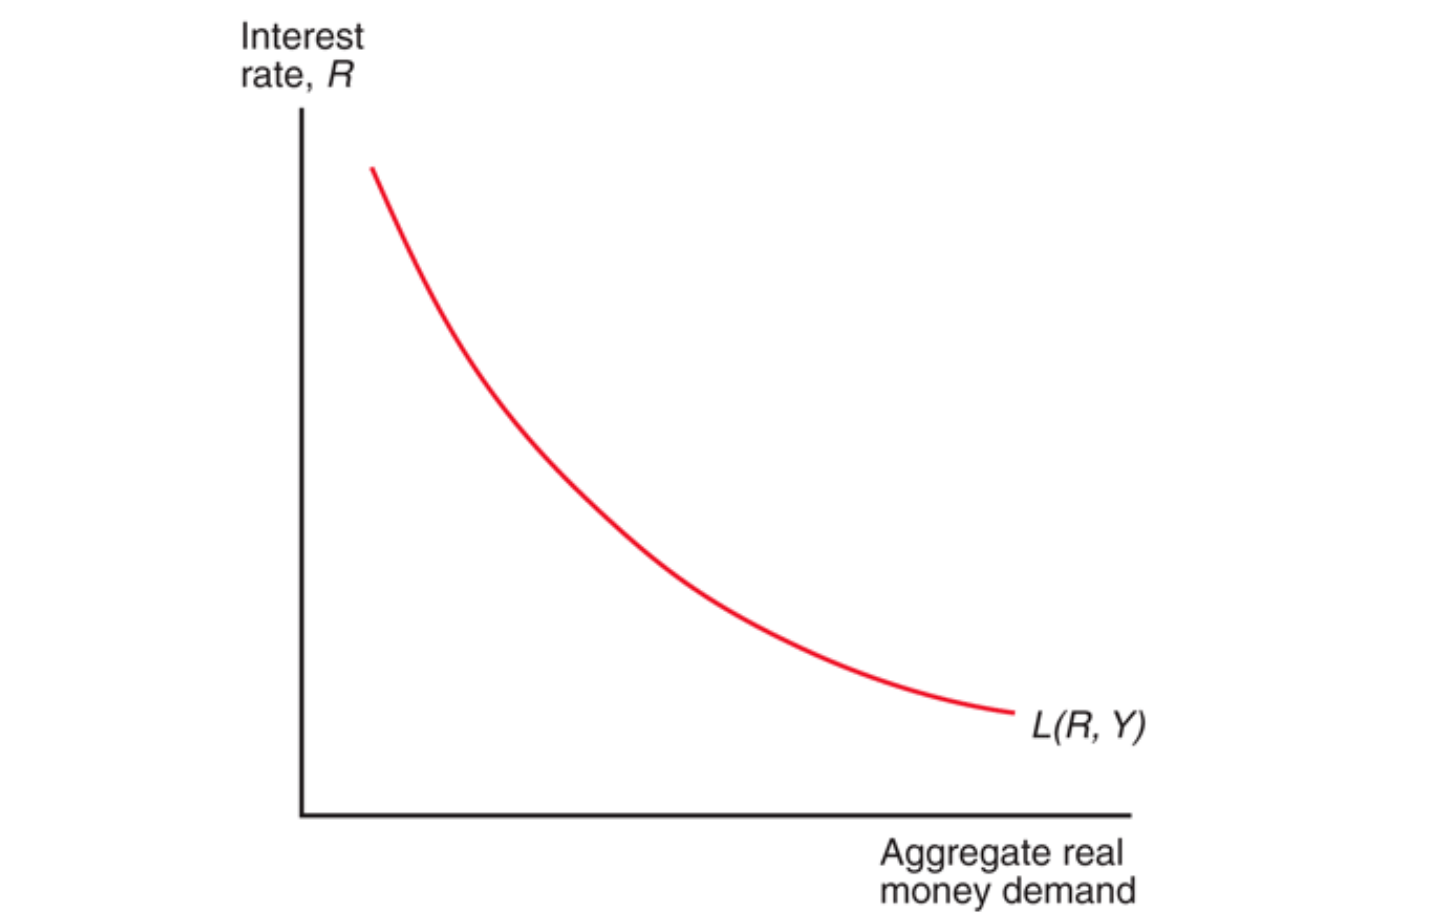
\includegraphics[scale=.15]{fig/shortrunexchange/int_demand.png}
\end{frame}

\begin{frame}{Shift in National Product}
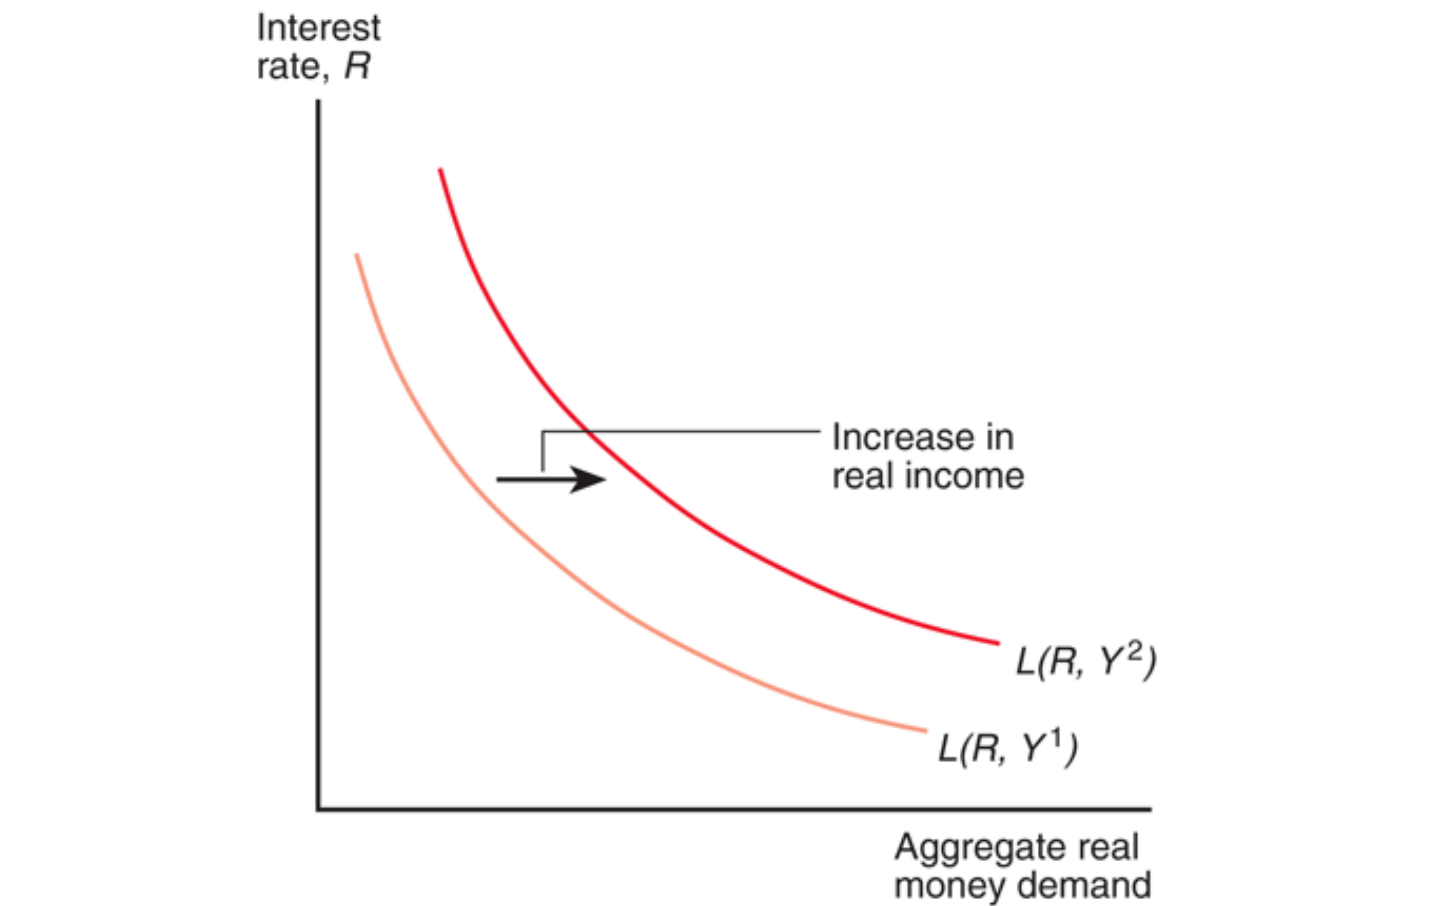
\includegraphics[scale=.15]{fig/shortrunexchange/GNP_shift.png}
\end{frame}

\frame{
\frametitle{A Short-run Model of the Money Market}
\begin{itemize}
\item Assume that changes in money supply do not affect:
\begin{enumerate}
	\item Price level
	\item GNP level
\end{enumerate}
\item Changes do affect interest rate of other assets
\item In equilibrium:
\begin{center}
	$M^{s}=M^{d}$
\end{center}
\item Plug in our formula for money demand, in equilibrium
\begin{center}
	$\frac{M^{s}}{P} =L\left(R,Y\right)$
\end{center}
\item Real money supply (LHS) equals real money demand (RHS)
\item Higher money supply $\Rightarrow$ lower interest rate
\end{itemize}
}

\frame{
\frametitle{Money supply and interest rate in the short-run}
\begin{itemize}
\item If more supply than demand for money:
\begin{enumerate}
	\item People with money will buy bonds for lower interest rate
	\item As interest rates fall, people more willing to hold money
\end{enumerate}
\item If more demand than supply for money:
\begin{enumerate}
	\item People will promise more money in the future for money today 
	\item As interst rates rise, people less willing to hold money
\end{enumerate}
\end{itemize}
}

\frame{
\frametitle{Determination of the Equilibrium Interest Rate}
\begin{figure}
\centering
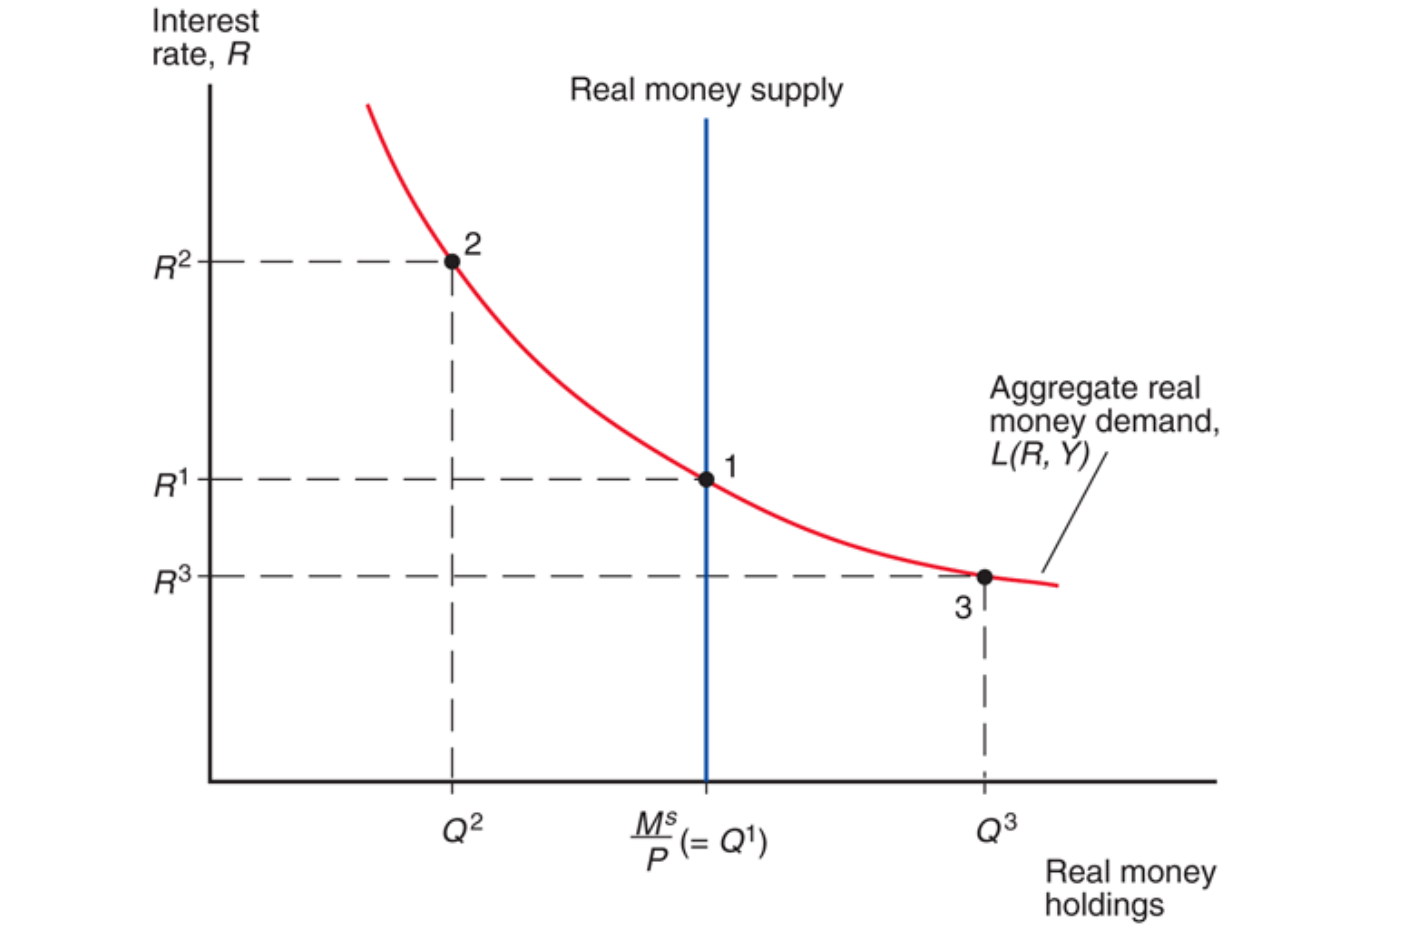
\includegraphics[scale=0.2]{fig/shortrunexchange/supply_demand.png}
\end{figure}
}

\frame{
\frametitle{Effect of an Increase in the Money Supply on the Interest Rate}
\begin{figure}
\centering
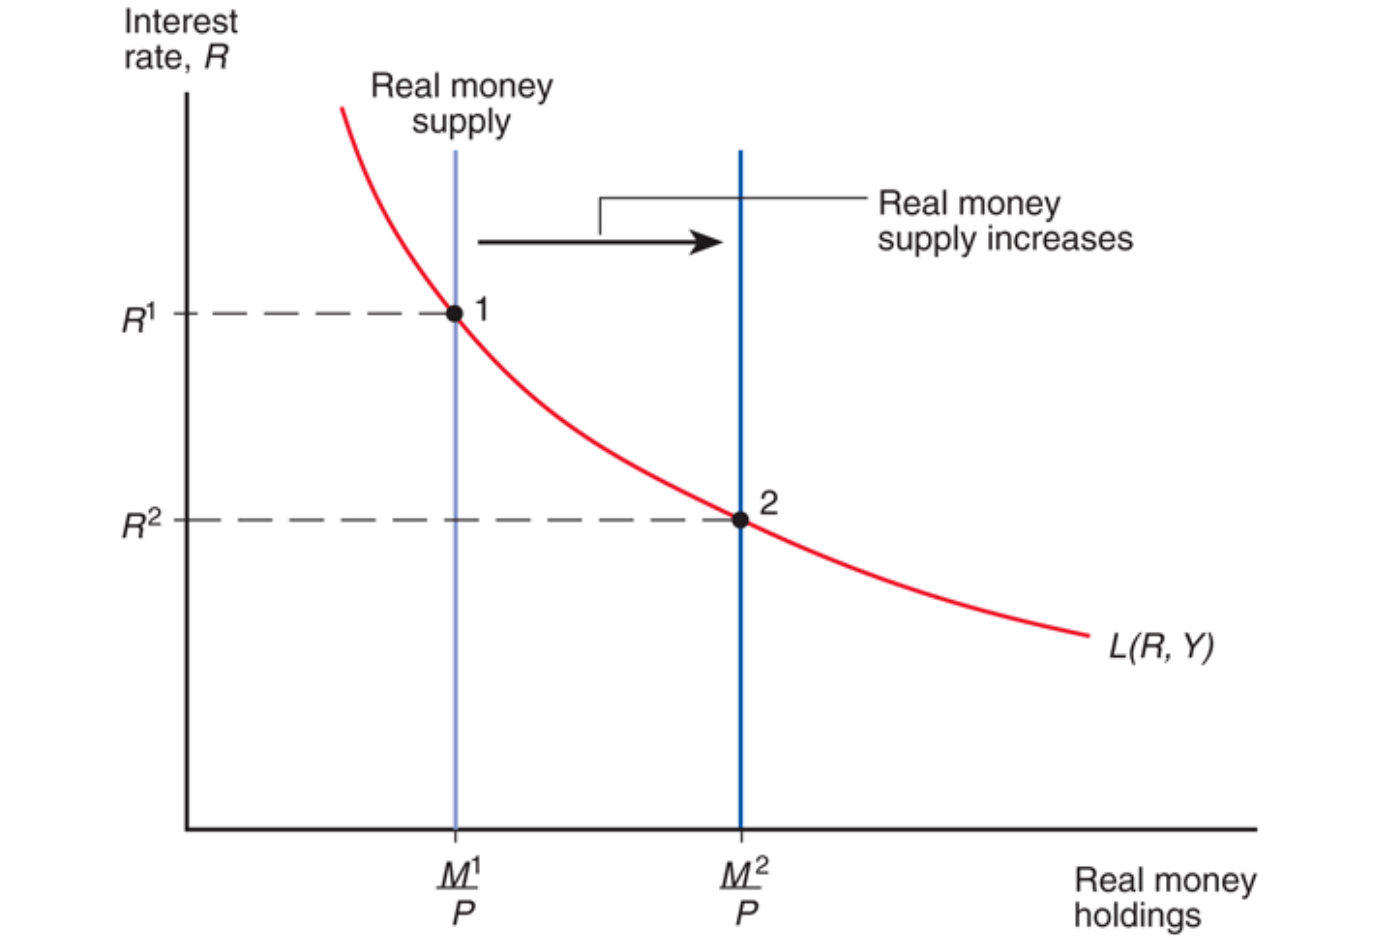
\includegraphics[scale=0.15]{fig/shortrunexchange/supply_interest.png}
\label{fig:11}
\end{figure}
\begin{itemize}
\item Short run: Central bank can lower interest rate by increasing money supply
\item Short run: Central bank can raise interest rate by decreasing money supply
\end{itemize}
}


\frame{
\frametitle{Effect on the Interest Rate of a Rise in Real Income}
\begin{figure}
\centering
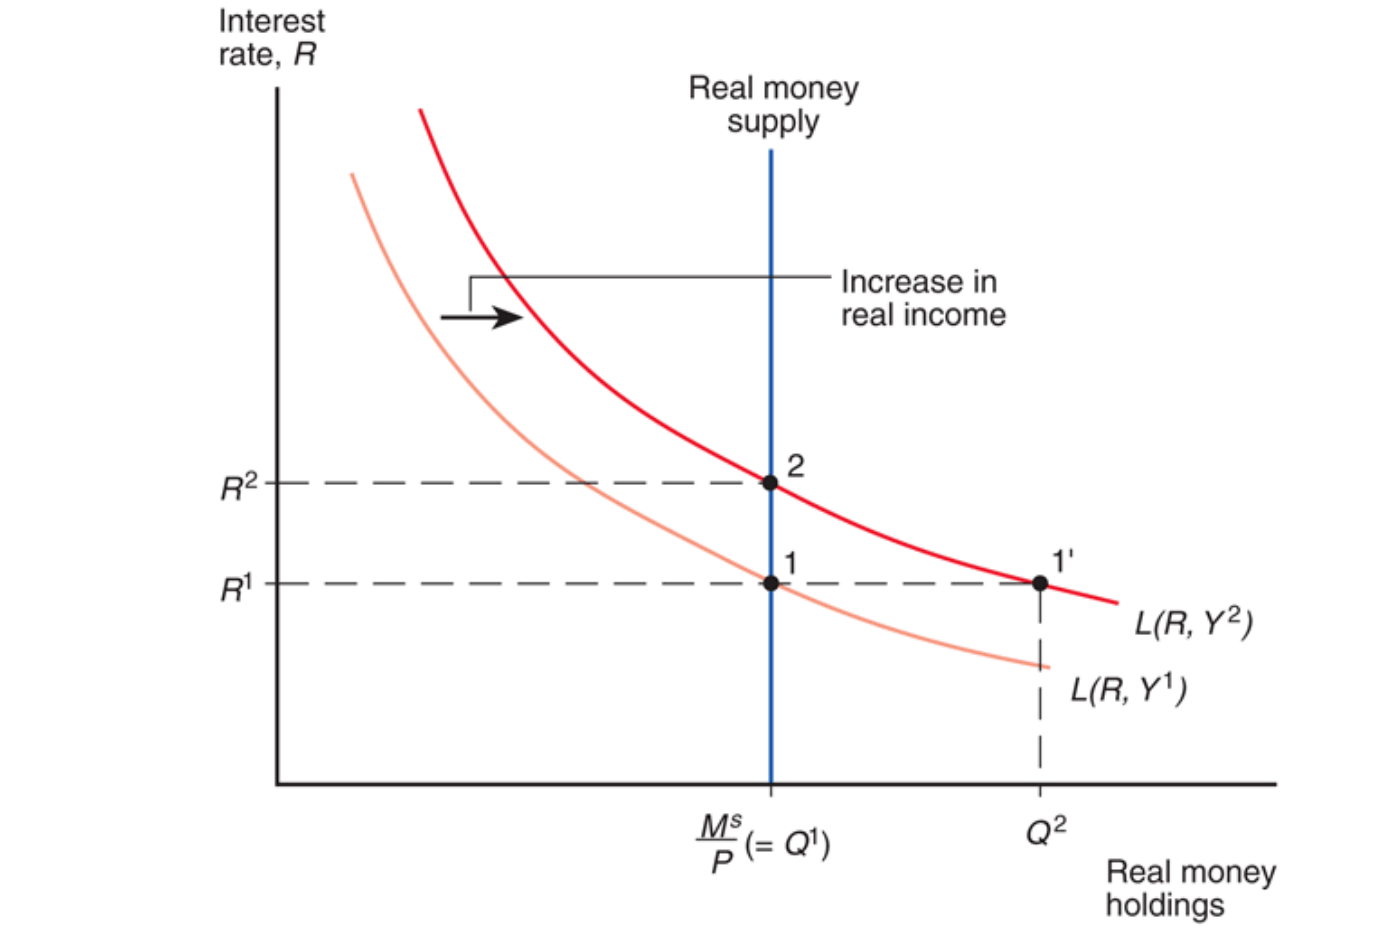
\includegraphics[scale=0.15]{fig/shortrunexchange/supply_real_income.png}
\end{figure}
\begin{itemize}
\item Short run: Output growth increases interest rate
\item Short run: A fall in output decreases interest rate
\end{itemize}
}

\begin{frame}{Reminder: Interest rate parity condition}

\begin{itemize}
\item Assume that the return on Euro bonds is fixed in Euros
\item Given dollar interest rate, exchange rate adjusts to satisfy parity 
\end{itemize}
\centering
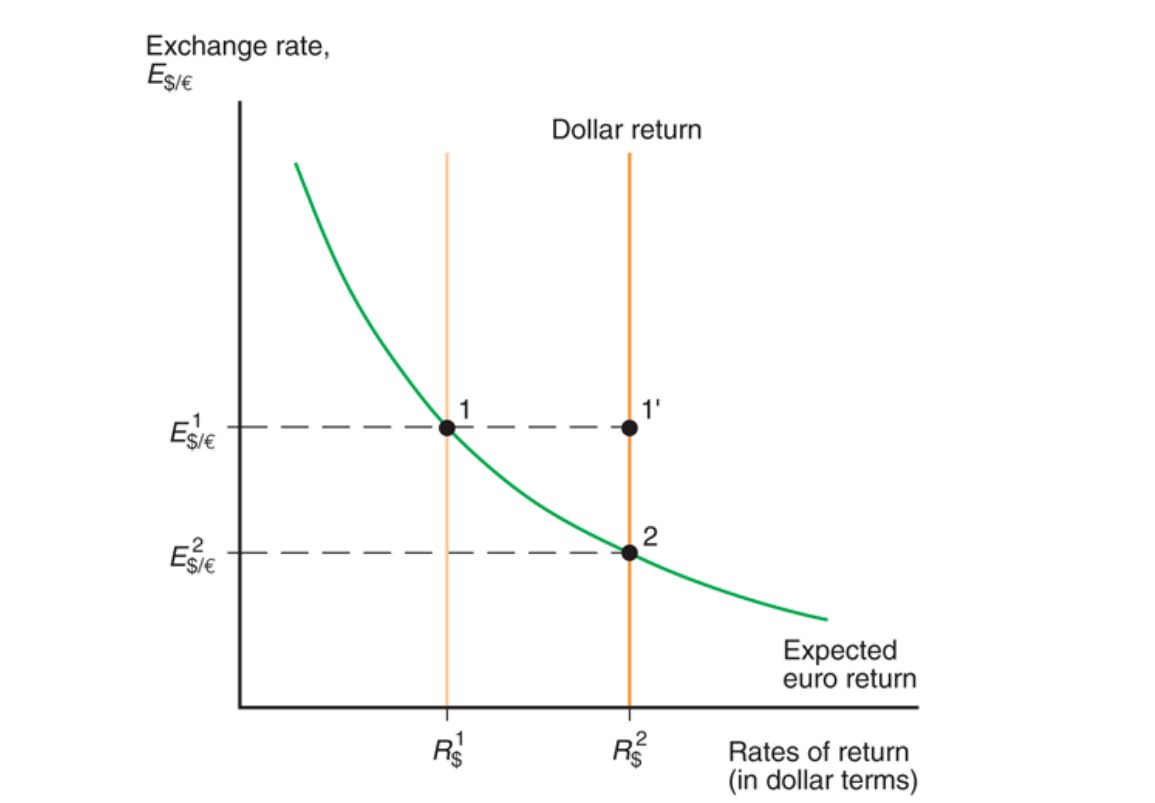
\includegraphics[scale=0.20]{fig/shortrunexchange/interest_rate_parity.png}
\end{frame}

\section{短期汇率理论2:粘性价格理论}

\begin{frame}{Money supply and exchange rate}

\begin{itemize}
\item Suppose Central Bank ups money supply
\item Interest rate goes down as people buy bonds
\item Dollar depreciates to maintain interest parity 
\end{itemize}
\end{frame}

\frame{
\frametitle{Money supply and exchange rate}
\begin{figure}
\centering
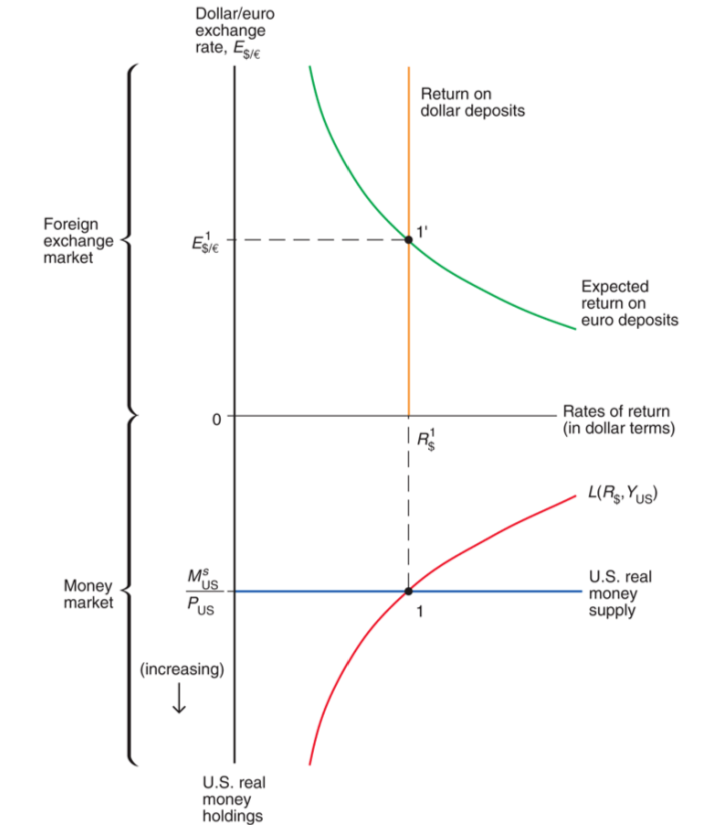
\includegraphics[scale=0.23]{fig/shortrunexchange/money_exchange.png}
\end{figure}
}

\frame{
\frametitle{Money Market/Exchange Rate Linkages}
\begin{itemize}
\item It is a two central bank game! 
\end{itemize}
\begin{figure}
\centering
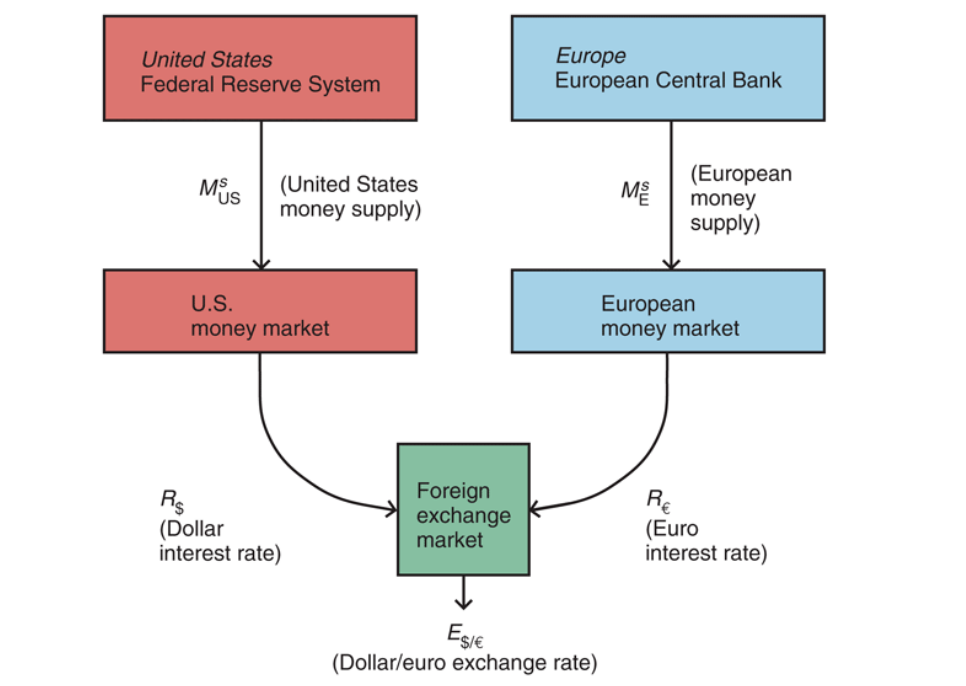
\includegraphics[scale=0.26]{fig/shortrunexchange/dollar_euro.png}
\end{figure}
}

\frame{
\frametitle{Increase in dollar supply}
\begin{figure}
\centering
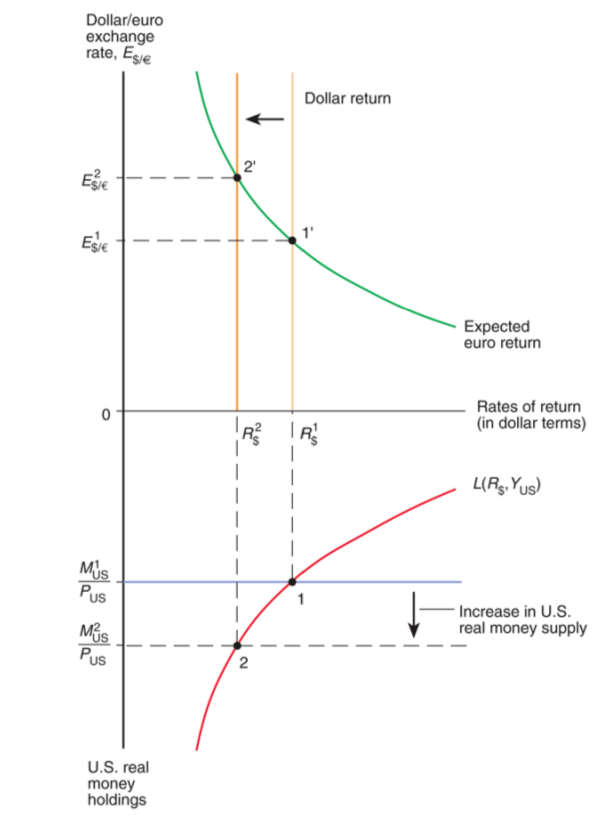
\includegraphics[scale=0.24]{fig/shortrunexchange/dollar_increase.png}
\end{figure}
}

\frame{
\frametitle{Increase in euro supply}
\begin{figure}
\centering
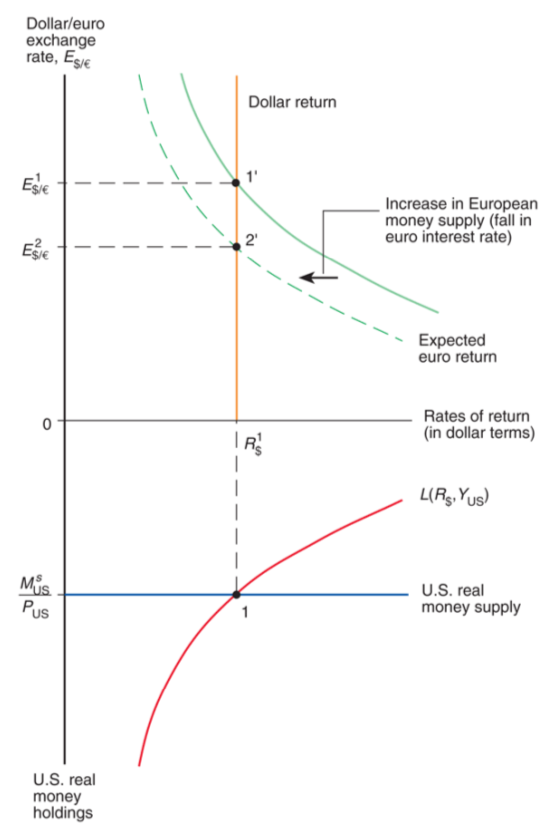
\includegraphics[scale=0.24]{fig/shortrunexchange/euro_increase.png}
\end{figure}
}



\frame{
\frametitle{Changes in the Domestic Money Supply}
An increase in a country's money supply:
\begin{itemize}
\item $R \Downarrow$
\item depreciation of the domestic currency
\end{itemize}
An decrease in a country's money supply:
\begin{itemize}
\item $R \Uparrow$
\item appreciation of the domestic currency
\end{itemize}
}


\frame{
\frametitle{Changes in the Foreign Money Supply}
How would a change in the supply of euros  affect the U.S. money market and foreign exchange markets?
\begin{itemize}
\item An increase in the supply of euros $\Rightarrow$ depreciation of the euro
\begin{enumerate}
\item $R_{EURO} \Downarrow$
\item depreciation of the euro
\end{enumerate}
\item A decrease in the supply of euros $\Rightarrow$ appreciation of the euro
\end{itemize}
}

\section{短期汇率理论3:弹性价格论}
\frame{
\frametitle{Long \& Short Run}
\begin{itemize}
\item Affect of more money supply
\item \textbf{Short run:} Prices are sticky, real money supply rises
\item \textbf{Long run:} Prices adjust so that real money supply falls to its original level
\end{itemize}
}

\frame{
\frametitle{In the Long Run}
In the long run, there is a direct relationship between the inflation rate and changes in the money supply.
\begin{itemize}
\item $M^{s} = P  L\left(R,Y\right)$
\item $P =\frac{M^{s}}{L\left(R,Y\right)}$
\end{itemize}
Money supply has no long run effecton output and interest rates
% \item $\frac{\Delta P}{P} = \frac{\Delta M^{s}}{M^{s}} - \frac{\Delta L}{L}$
% \end{itemize}
% The inflation rate is predicted to equal the growth rate in money supply minus the growth rate in money demand.
}

\frame{
\frametitle{Money supply, output and interest}
\begin{itemize}
\item Money supply has no long run effection on output and interest rates
\item Intuition
\begin{itemize}
\item A currency reform: Turkish millionaires
\item 2005, new Turkish lira, divide old lira by one million
\item For a period, both lira could be used
\item Everything in the country lost six zeros
\item No effect on output or interest
\end{itemize}
\item Central Bank actions are similar
\item Double the money, halve the prices
\end{itemize}
}


\frame{
\frametitle{Money supply, demand, and inflation}
\begin{itemize}
\item Long run prices:
\item $P =\frac{M^{s}}{L\left(R,Y\right)}$
\item $\frac{\Delta P}{P} = \frac{\Delta M^{s}}{M^{s}} - \frac{\Delta L}{L}$
\end{itemize}
The inflation is the growth rate in money supply minus the growth rate in money demand.
}

\frame[plain]{
\frametitle{Average Money Growth and Inflation in Western Hemisphere Developing Countries, by Year, 1987-2007}
\begin{figure}
\centering
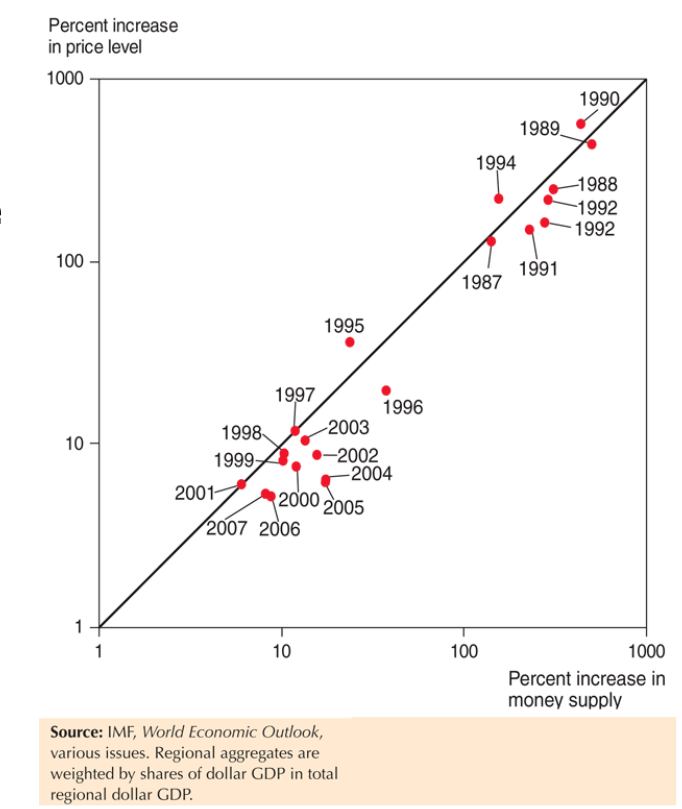
\includegraphics[scale=0.28]{fig/shortrunexchange/inflation_supply.png}
\label{fig:11}
\end{figure}
}

\section{长期+短期:汇率超调}

\frame{
\frametitle{Short run and Long run}
\begin{itemize}
\item Money cannot shift prices immediately
\begin{itemize}
\item Long-term contracts
\item Menu costs
\end{itemize}
\end{itemize}
}

\begin{frame}{Exchange Rates vs Price Level}
\begin{itemize}
\item In short-run example, we let exchange rates adjust, not prices;
\item This assumption seems reasonable for US and Japan
\end{itemize}
\centering
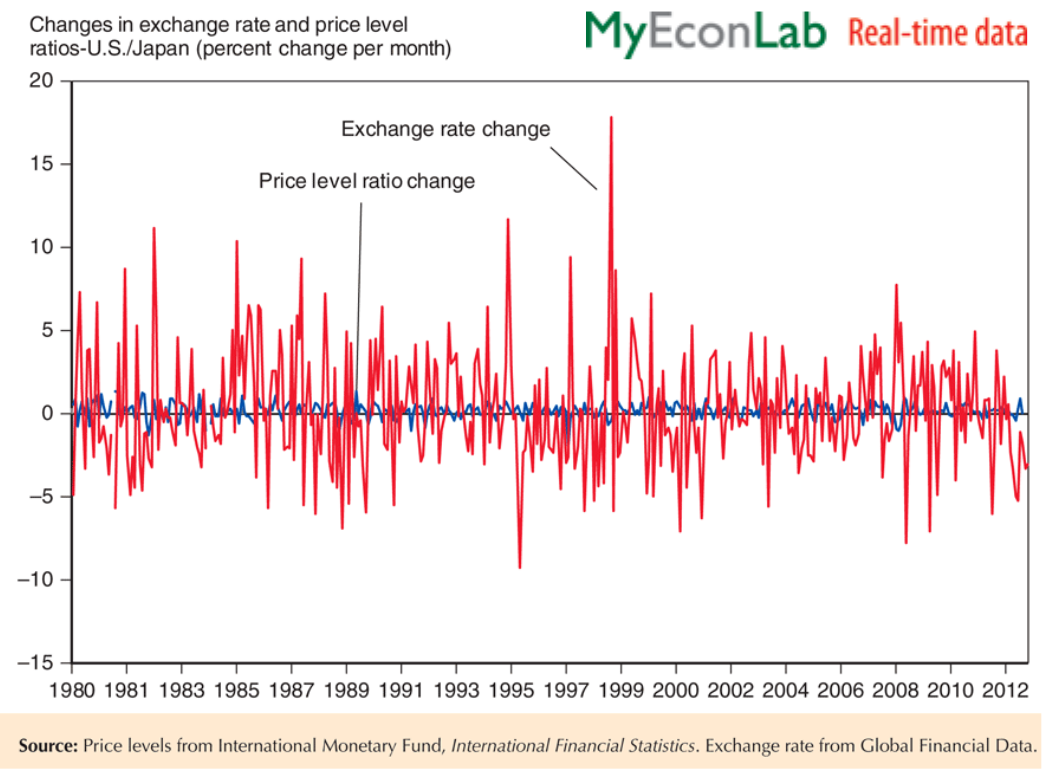
\includegraphics[scale=0.23]{fig/shortrunexchange/us_japan_prices.png}
\end{frame}

\frame{
\frametitle{Short run and Long run}
\begin{itemize}
\item Money cannot shift prices immediately
\item Over time, however, prices will adjust
\begin{enumerate}
\item Excess demand of goods and services: labor $\Uparrow$ $\Rightarrow$ wage $w \Uparrow$  $ P \Uparrow$
\item Inflationary expectations: $P^{e} \Uparrow w \Uparrow P \Uparrow$
\item Raw materials prices: Adjust quickly
\end{enumerate}
\end{itemize}
}

\frame[plain]{
\frametitle{Excess demand for factors}
\begin{itemize}
\item More money but the same prices means people buy more
\item To produce more, firms have to buy more inputs
\item Old workers are stuck on contract
\item New workers can bargain for higher wages
\item The increase in input price causes increase in output price
\end{itemize}
}

\frame[plain]{
\frametitle{Inflationary expectations}
\begin{itemize}
\item People know about increse in money supply 
\item Long run, prices will rise
\item Workers bargaining for Long-term contracts will demand higher wages
\end{itemize}
}

\frame[plain]{
\frametitle{Raw materials}
\begin{itemize}
\item The price of raw materials (oil) adjusts quickly
\item Output prices eventually need to reflect increase in input cost
\end{itemize}
}

\begin{frame}{Money supply and exchange rates, long-run}
\begin{itemize}
\item Review: 
\begin{itemize}
\item The return to Euro bonds in dollars depends on expected depreciation
\item The more the dollar is expected to depreciate, the higher Euro bond returns
\end{itemize}
\item Permanent money supply increases raise expected depreciation
\end{itemize}
\end{frame}



\begin{frame}{Increase in money supply and exchange rate, long-run}
\begin{itemize}
\item Initially:
\begin{itemize}
\item Money supply goes up, interest rate falls, depreciation
\item Money supply goes up, expected depreciation, more depreciation
\end{itemize}
\item Then:
\begin{itemize}
\item Prices adjust to long run real money supply level
\item Real money supply falls, interest rate rises, appreciation
\item Exchange rate settles level depreciated relative to initial level
\end{itemize}
\item The double depreciation followed by appreciation: \emph{exchange rate overshoot}
\end{itemize}
\end{frame}

\frame{
\frametitle{Money, Prices, Exchange Rates, and Expectations}
\begin{figure}
\centering
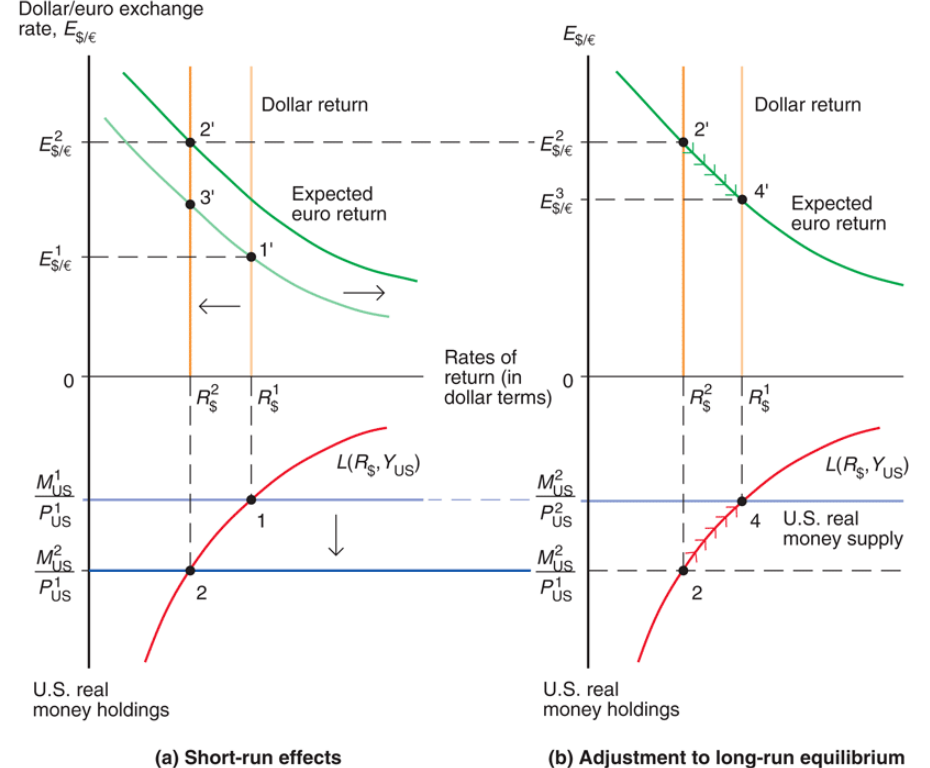
\includegraphics[scale=0.25]{fig/shortrunexchange/long_run_exchange.png}
\end{figure}
}

\frame[plain]{
\frametitle{Money, Prices, Exchange Rates, and Expectations}
\begin{figure}
\centering
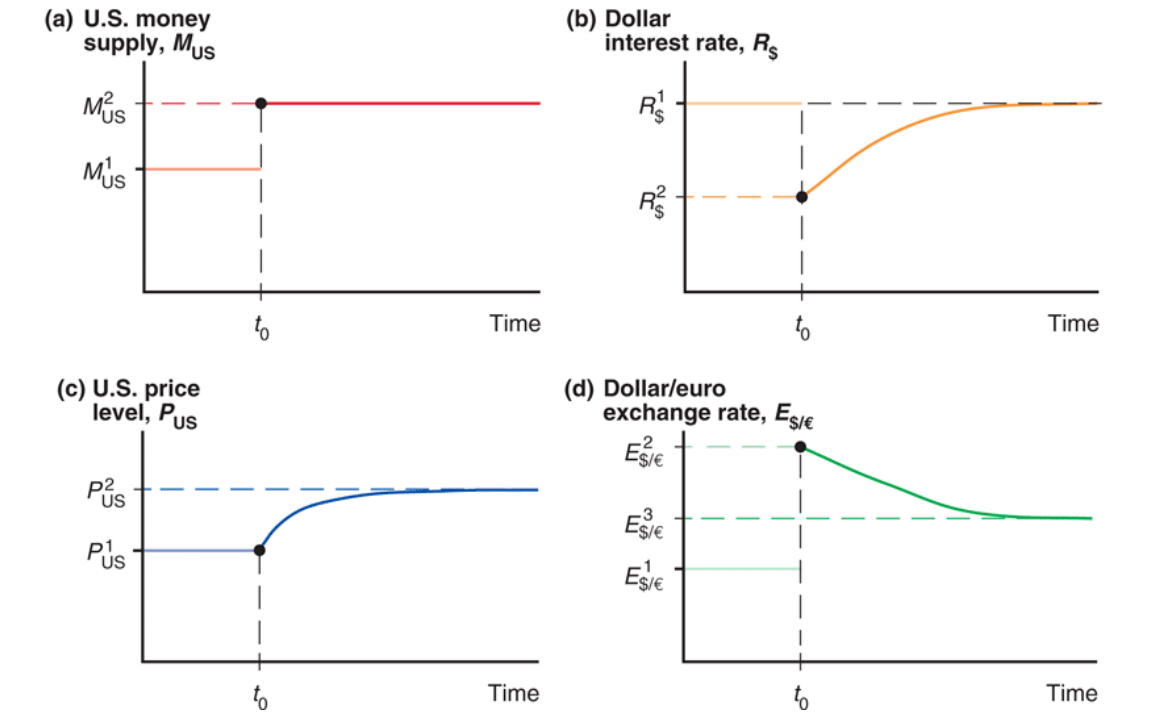
\includegraphics[scale=0.27]{fig/shortrunexchange/macro_impulse.png}
\label{fig:11}
\end{figure}
}

\begin{frame}{Summary of Chapter 15}
\begin{itemize}
\item We have seen short run sticky prices which cause short-run real effects
\item We have seen that in the long run, money is neutral (no real affect)
\item We have seen that expectations about money supply affect current exchange rates
\item In Chapter 16, we will study how long-term demand and supply shifts affect exchange rate
\item Discussion builds on the linkages studied in Chapter 15
\end{itemize}
\end{frame}

\end{document}
